\chapter{Foundation}

A literature survey on the topic of augmented reality in maritime context brings up studies of applications that aid job performance by providing helpful contextual information on top of real-world views. Overlaying route waypoints, distance to next waypoint, local hazards and other navigational aids allows the integration of various information that is used by the officer of the watch into one single augmented display. In poor visibility conditions, virtual rails on both sides of the ship help with steering. Buoys, fog signals, day beacons and other navigational aids can also be visually overlaid in low-visibility conditions to help with navigation. These applications show the use of augmented reality as aids for task execution. But little research can be found on use in training ship crew.

This chapter covers results of a domain analysis that was used to derive requirements for a scenario-based ship maneuvering training method. The content explored in this chapter are relevant to answering the research question - what are the operational scenarios in which mixed reality training could be useful. In keeping with the sCE method, it covers operational demands, human factors and, technological options available for the design of this human-computer interface for maritime training. 

The first section is an introduction to ship handling in general, including a specific case - the offshore energy industry where unique requirements led to the development of increased automation and specialised equipment for manoeuvring. Section \ref{sec:operationaldemands} titled operational demands describe from an operator point-of-view, requirements for safe execution of ship handling operations. In designing a technological solution, the SCE method takes into account human factors that could affect interactions between users and the system being developed. Section \ref{sec:humanfactors} titled human factors knowledge describes mode errors - a type of error arising from the operation of state-dependent systems out of state. Finally, section \ref{sec:envisionedtech} describes technological options available to implement the mixed reality training method that is envisioned along with their pros and cons.



\section{Ship Handling}

Given the varied environments in which ships are handled, a distinction is made between vessel handling in restricted spaces as opposed the same in open seas with vast empty space. Manoeuvring typically refers to handling of ships in confined spaces and at low speeds; requiring accuracy and precision in movement. In contrast, navigation occurs in open seas with more room for movement which makes it a comparatively easy task over maneuvering. Besides, a ship usually moves in straight lines while navigating the open seas with the objective to reach destination in the most efficient manner. Fewer changes in direction occur over time, there is lesser need to steer in comparison with manoeuvring scenarios. 

Automation has been seeping into the marine industry over the years. It assists human operators to accomplish vessel handling tasks with functions such as autopilot for navigation and dynamic positioning for maneuvering. The underlying idea is to counter water resistance to movement using the ship's propellers and thrusters, while also accounting for environmental forces such as wind, waves and current measured using sensors on board. Current generation autopilots do a satisfactory job of navigating ships in open seas. Maneuvering on the other hand continues to be a specialized human job even though a good degree of automation support exists.

% Hence, this research focuses on training for ship maneuvering. 

The training method developed here is aimed at learning maneuvering. Besides being a skilled task, it also involves safety risks by nature of its activities. The next section describes challenges of maneuvering and its relevance in the offshore oil industry. It is followed by a brief description of Dynamic Positioning Systems, the automation technology that assists with ship maneuvering tasks and its riders that entail the presence of operators with manual handling skills. 

\subsection{Maneuvering}

Vessel handling at low speeds has been difficult on marine vessels historically \parencite{brittanica:ship}. From a technical point of view, the working mechanism of past rudder systems made it difficult to turn vessels 'in place'. Maneuvering a large vessel at low speeds is often a challenging operation even from the perspective of a human operator. Examples of difficult maneuvering operations include approaching a harbour, berthing in a port, sailing side-by-side another vessel, approaching and stationing close to an oil platform, etc. An often recurring sequence is that of a port-bound vessel heading to its berthing location in harbour. Having entered pilot waters from seaward, a vessel's course needs to be controlled accurately to ensure safe passage through channels, bridges, and locks; avoiding collisions with other vessels at the same time. A method for objective evaluation of ship handling difficulties in restricted maneuvering area, areas of traffic congestion is presented in \parencite{inoue2000evaluation}.

Many factors affect the precise handling of a given vessel - it's size, power, thruster configuration, on-board bridge equipment, etc. Further, the vessel's handling characteristics are subject to environmental conditions (the combined effect of current, wind and, waves). Besides, low speed maneuvering often occurs in close proximity to man-made constructions such as docks, offshore structures and other ships. The potentially destructive consequences of collision risks in such scenarios makes it a stressful operation, further amplifying the challenge of maneuvering. Safety risks involved in such tasks make it a stressful operation. Mistakes have high associated costs, possibly leading to lost lives and damage to expensive constructions.

\subsection{Offshore Supply Operations}

A special application of ship handling skill is on-board offshore supply vessels. These are vessels that are used in support of exploration and production of offshore mineral or energy resources located in continental shelves around the world. Specific missions of offshore supply vessels include 
\begin{itemize}\renewcommand{\labelitemi}{\tiny$\blacksquare$} 
\item seismic survey to locate potential oil and gas fields
\item towing of rigs to their location, positioning them and laying anchoring and mooring equipment
\item supplying equipment, personnel, provisions, other necessary goods to rigs
\item subsea operations such as ROV operation, diving support, inspection and maintenance
\item safety standby for emergency response and rescue operations
\end{itemize}

Maneuvering plays an important role in platform supply vessels. They transport supplies such as fuel, water and chemicals to the offshore facilities and bring back disposables for proper recycling. Hence, these vessels need to approach and be stationed close to platforms on a regular basis. Loading and unloading operations happen at the stern of a vessel and requires station keeping till the operation is complete. This requirement led to the development and subsequent popularity of dynamic positioning systems. These are automated systems that help with station keeping and other maneuvering operations. The following sections describe the dynamic positioning system, their conceptual working mechanism and modes of operation before making a case about the need for skilled manual maneuvering operators.

\begin{figure}
	\centering
	\caption{Prominent oil and gas fields in the North sea}
	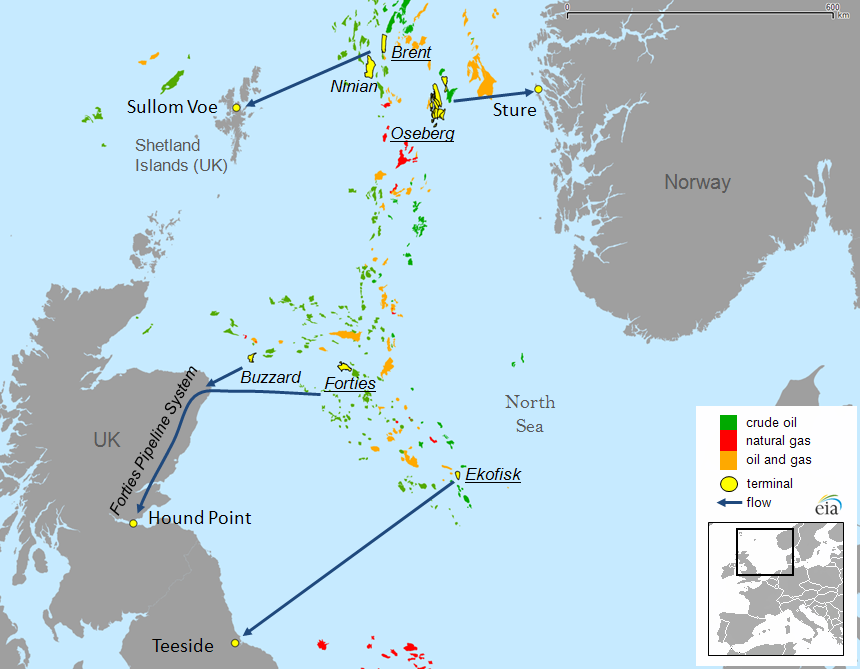
\includegraphics[width=\linewidth]{northseamap}
	%\todo[inline]{Get higher resolution picture}
	\label{fig:northseamap}
	\hbox{\small Source: \thinspace{refer footnote\protect\footnotemark}}
\end{figure}
\footnotetext{U.S. Energy Information Administration, United Kingdom Department of Energy and Climate Change, Norwegian Petroleum Directorate}

\subsubsection{Dynamic Positioning System}

Dynamic positioning (DP) is an automated system that helps human operators with maneuvering operations. It began to be developed as a system that maintains position and heading of a vessel automatically by using its propellers and thrusters. The use of DP systems has been increasing over the years since its inception in 1960s. There are well over 2000 DP vessels in operation today \cite{sorensen2011survey}. From early days of the technology where main focus areas of research were accurate position measurement and control system technologies used, research has now moved on to more specialized problems such as optimizing them for energy efficiency. With increasing popularity of DP systems and increased use of sophisticated technology onboard ships, the marine industry can expect more advanced automation in vessel control over the years. Future systems could be enabled with features such as automatic maneuvering in shallow water and harbor areas, formation sailing, and automatic collision avoidance.

%The popularity of DP systems has grown to a point where they are a component of medium to large sized vessels these days. 

%This evolution of navigation technology on ships from mere position monitoring systems to automatic position control system has been accompanied by a corresponding growth of specialized personnel responsible for the monitoring of DP systems. 

Information from position reference sensors that provide the vessel’s position and heading, along with information from wind sensors, motion sensors and gyrocompasses on the vessel are used by the system. It is supplied as input to a program that calculates changes in position, heading required to bring the vessel a preset location by activating the vessel’s thrusters when necessary. Using a mathematical model of the ship and, the forces acting on it, the DP system can control the vessel's thrusters to position it in a preset destination.

% Figure \ref{fig:dparchitecture} is a model of the functional components of a dynamic positioning system. 
%
%\begin{figure}
%	\centering
%	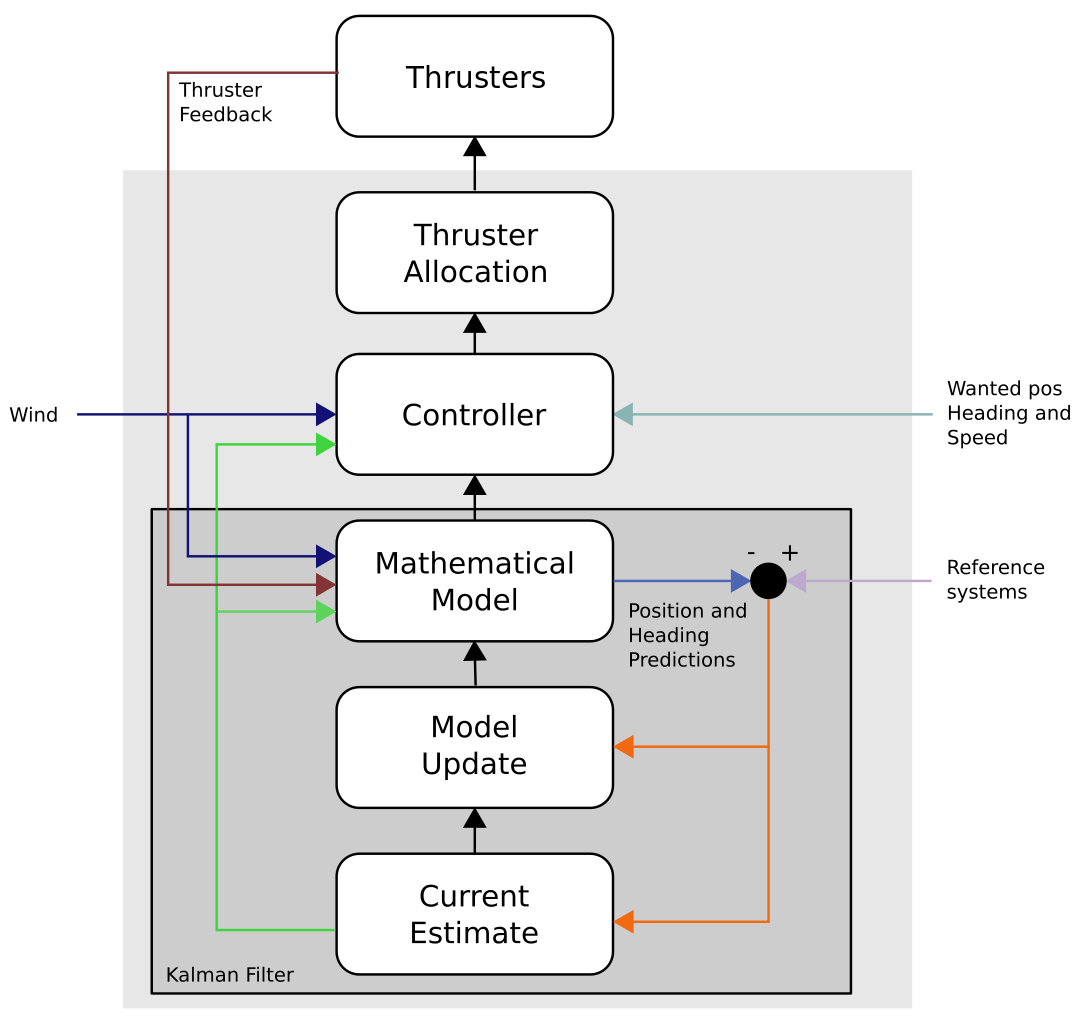
\includegraphics[scale=0.35]{dparchitecture}
%	\caption{Model architecture of Dynamic Positioning systems}
%	\label{fig:dparchitecture}
%\end{figure}
%
%The system contains a \textit{controller} module that influences vessel movements by taking decisions on power allocation for individual vessel thrusters. It takes as input, weather information from wind sensors and current position information from position reference systems. Expected output is to position the vessel at a position and heading preset by the operator. After being initiated, the system determines the difference between current position and desired position. It then attempts to minimize this difference over time. This is done by firing appropriate thrusters into action, producing vessel movements in different directions. 

\begin{figure}
	\centering
	\caption{Forces acting on a ship and its possible movements}
	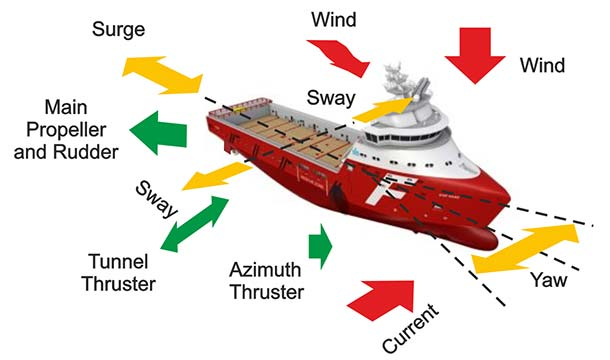
\includegraphics[scale=0.60]{dynamic-positioning}
	\hbox{\small Source: \thinspace{kongsberg.com}}
	\label{fig:shipforces}
\end{figure}

The system needs to compensate for unpredictable environmental forces as it decides on allocations for individual thrusters. While the system takes into account wind forces acting on the vessel measured using wind sensors, as shown in \ref{fig:shipforces}, a vessel's position is also affected by ocean currents and waves. Kalman filter is generally used to model the environmental forces. It is an algorithm that uses a series of measurements observed over time, containing statistical noise and other inaccuracies, and produces estimates of unknown variables by using Bayesian inference and estimating a joint probability distribution over the variables for each timeframe. While it tends to be more precise than algorithms based on a single measurement alone, it is a nevertheless a probability based system that produces estimate predictions of changes in environmental forces over time and some uncertainty in predictions can be expected. Although there do not exist rules specifying acceptance criteria for the positioning performance of DP systems, DNVGL guidelines state that "in moderate weather conditions and with a fully operational DP-system the vessel should generally be able to demonstrate position keeping accuracy with a 3 meter radius and $ \pm $ 1\degree of heading." \parencite{veritas2011dynamic} 



%\todo[inline]{write about accidents that occured. ekofisk etc}

%Figure \ref{fig:praxisdp} shows the interface of a typical DP system. A display monitor is used to show various information regarding the vessel and its control systems. Apart from the display, there exists input interface in the form of buttons. They are used to provide information to the system such as desired location and the mode in which it will be used. 

\paragraph{Dynamic Positioning Modes}
Most DP systems are offered with several modes of operation. They differ in the type of operation and amount of automation involved. Following are a few common modes of operation. 

%\begin{figure}
%	\centering
%	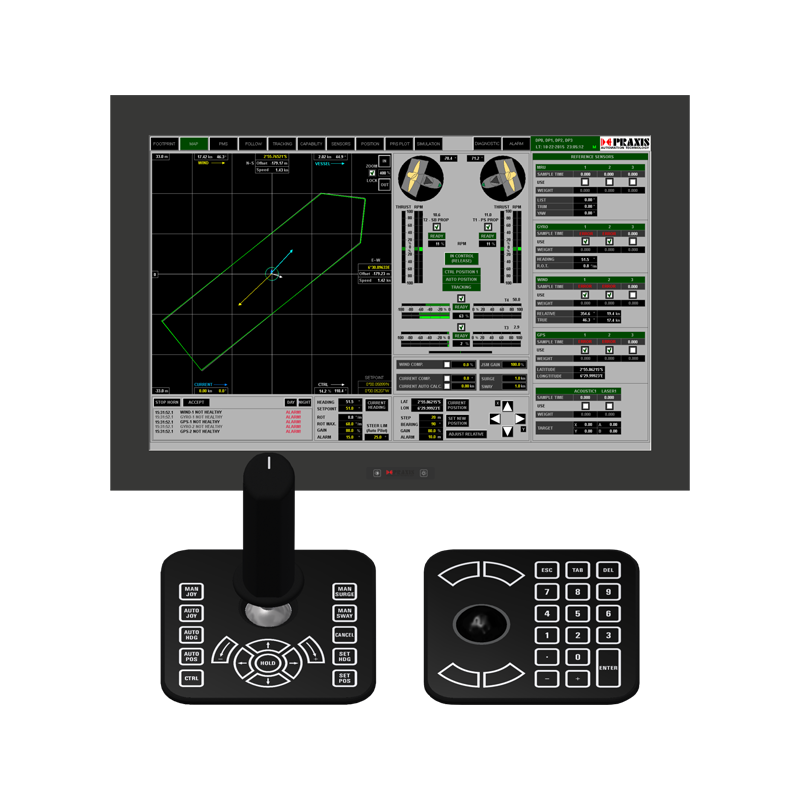
\includegraphics[scale=1]{praxisdp}
%	\caption{Typical dynamic positioning console}
%	\label{fig:praxisdp}
%\end{figure}

\begin{enumerate}

\item \textbf{Joystick}: In this mode, the operator can control the vessel position and heading manually using a joystick. 
\item \textbf{Auto heading}: In this mode, the vessel automatically maintains a preset heading. 
\item \textbf{Auto position}: This mode automatically maintains the vessel's position and heading. 
\item \textbf{Follow target}: Enables the vessel to automatically follow a moving target. 
\item \textbf{Autopilot}: In this mode, the vessel steers automatically to follow a predefined course. 

\end{enumerate}

It can be observed that besides functionality, the modes listed above differ by the level of automation involved in the functionality. The joystick mode offers the least amount of automation. In this mode, a single lever can be used to control all of the vessel's thrusters at the same time. A large vessel such as a platform supply vessel typically has two azimuth thrusters at the stern-end of the vessel and one at the bow-end. In addition, they also typically have tunnel bow thrusters that can be used to turn the vessel in place. While it is possible to control each of the thrusters individually from the bridge of the vessel for fine-grained control; the joystick mode encapsulates all the thrusters into one control. This allows control of forward, reverse, steering and even sideways motion using just one lever. 

%\begin{figure}
%	\centering
%	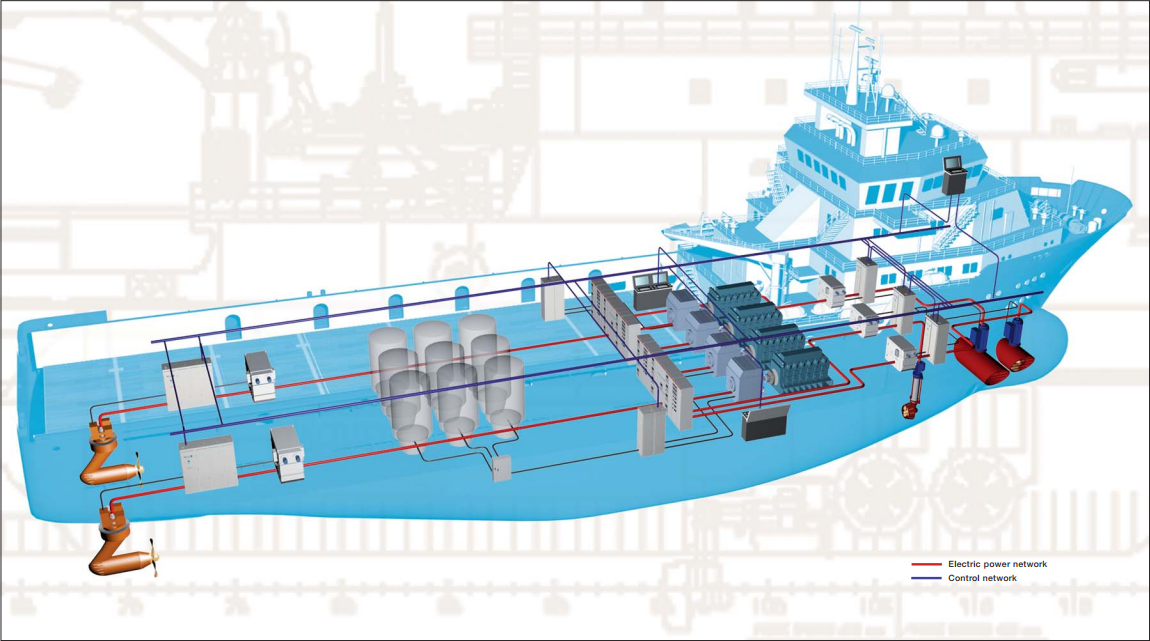
\includegraphics[scale=0.45]{osvlayout}
%	\caption{Schematic diagram of the power and control network of a typical offshore supply vessel}
%	\label{fig:osvlayout}
%\end{figure}

\subsubsection{Manual Handling}
Going by number of total losses occuring per year (refer figure \ref{fig:lossesbyyear}), the safety of vessels world-wide can be said to have improved over the years, particularly the last decade, despite the ever increasing number of sea-faring vessels. Nevertheless, there is a growing concern in the industry regarding over-reliance on electronic navigation aids. Studies have found human error to be dominant factor in a significant percentage of the accidents \parencite{baker2005accident, hauff2014analysis}. Incidents such as the Norne shuttle tanker's collision with an FPSO on 5 March 2000, Big Orange XVIII's collision with the water injection facility Ekofisk 2/4-W on 8 June 2009 and standby vessel Far Symphony's impact with the mobile installation West Venture on 7 March 2004 are mentioned as cases of shipping incidents that showcase the lack of preparedness among crew members to handle with emergency situations \parencite{vinnem2013offshore}.

\begin{figure}
	\centering
	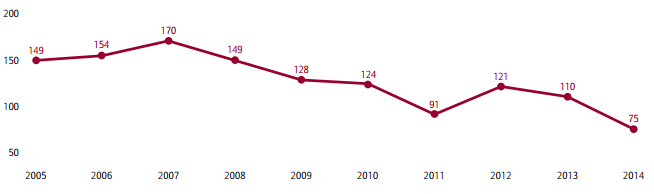
\includegraphics[scale=0.75]{lossesbyyear}
	\caption{Yearly vessel loss since 2005}
	\label{fig:lossesbyyear}
\end{figure}

\section{Operational Demands}
\label{sec:operationaldemands}
An intuitive understanding of the vessel’s handling is required to manually manoeuvre the vessel. Different vessels exhibit different handling behavior depending on their propulsion technology, steering controls, and, dynamics of the particular vessel, owing to its design. These factors have a combined effect on the handling behavior of the vessel, that is unique to the vessel, or the vessel type in general. Besides, vessels also differ in the way they respond to various weather conditions. 
Gaining a high level of intuitive understanding of the vessel’s motion dynamics comes with extensive practice. A manoeuvre training system should then enable maneuvering practice on the real vessel in real situations.

A clear view of the target object around which the vessel is being maneuvered provides direct visual feedback of the target’s position relative to the vessel. By looking out the bridge windows, the operator can immediately learn about the progress of the maneuvering operation. Using this information, the operator can make adjustments to the vessel's movement as required. When maneuvering large vessels, besides the person at the helm, another person usually aids the operation. Standing outside the bridge of the vessel, this person keeps a lookout for the position of the ship, and conveys it to bridge personnel. He also keeps a lookout for traffic and other objects in the vicinity such as navigational aids.

Figure \ref{fig:nidpcertification} shows the certification process required to be a qualified dynamic positioning operator. One starts with a classroom-based induction course that provides basic knowledge of the principles and practical use of DP. After such a course, the trainee is expected to be familiar with the components of a DP system, concept of redundancy that separate different classes of DP systems, its modes of operation and limitations. Thereafter the trainee goes on to acquire watchkeeping experience onboard real vessels with DP. This watchkeeping exercise takes place for a relatively short period of time where the trainee is familiarised with DP equipments onboard the vessel and gets to witness operations. This is followed by a simulator-based course where the trainee gets practical experience operating DP systems in onshore simulation centers. 

\begin{figure}
	\centering
	\includegraphics[scale=0.75]{nidpcertification}
	\caption{Flowchart of nautical institute Dynamic positioning certification scheme}
	\label{fig:nidpcertification}
\end{figure} 

\section{Human Factors Knowledge}
\label{sec:humanfactors}
\subsection{Mode Errors}
Mode errors are the errors that occur when a user operates an interface in a manner that is appropriate to a different state of the system than the one it actually is in. When the user forgets the actual state and performs an action appropriate to a different state, the system response is unexpected and usually undesired. A common example of mode errors is the undesired input of capitalised letters on a computer due to caps lock, or the inability to enter numbers using the number pad due to numlock. 

The design of a ship operation training method set in augmented reality needs to take into account the possibility of mode errors resulting from the two realities that are simultaneously at play. A trainee moving a real ship in augmented reality is also moving it in reality. Take the example of a training exercise to approach a virtual object out in the open sea. In the course of the exercise, the trainee moves the vessel towards the virtual object in the augmented reality. At the same time, the real vessel is actually moving somewhere out in the open sea. If the bridge equipment is also augmented, the radar would be expected to display an indication of the virtual oil platform. Adding a virtual object to a radar display that already contains information regarding other real objects can be confounding to users. A way to distinctly identify virtual objects should help reduce mode errors but it also hampers immersion of the experience. 
It is advised to avoid the possibility of mode errors when possible (citation needed). 

\begin{figure}[ht]
    \centering
    \begin{subfigure}[b]{0.45\textwidth}
        \centering
        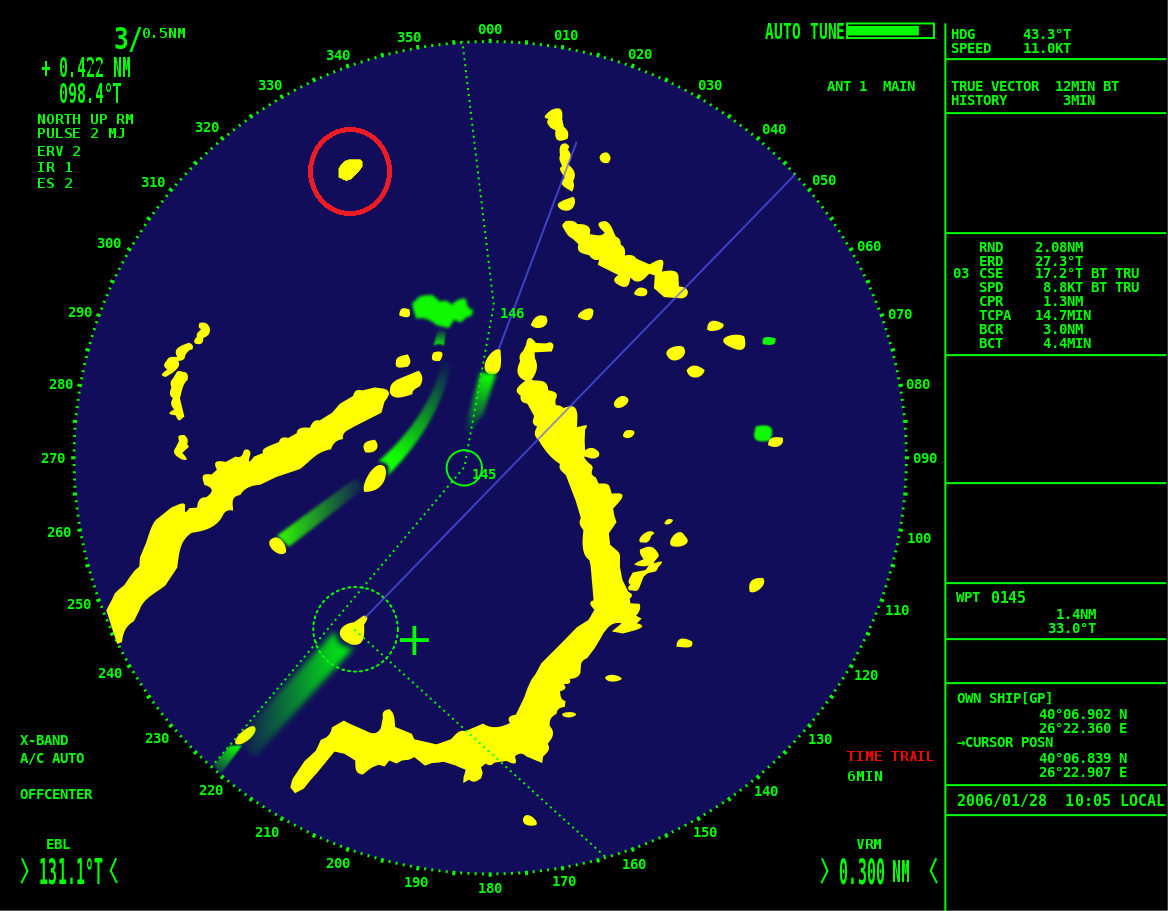
\includegraphics[width=\textwidth]{radarOrig1}
        \caption{No colour differentiation}
        \label{fig:three sin x}
    \end{subfigure}
    \hfill
    \begin{subfigure}[b]{0.45\textwidth}
        \centering
        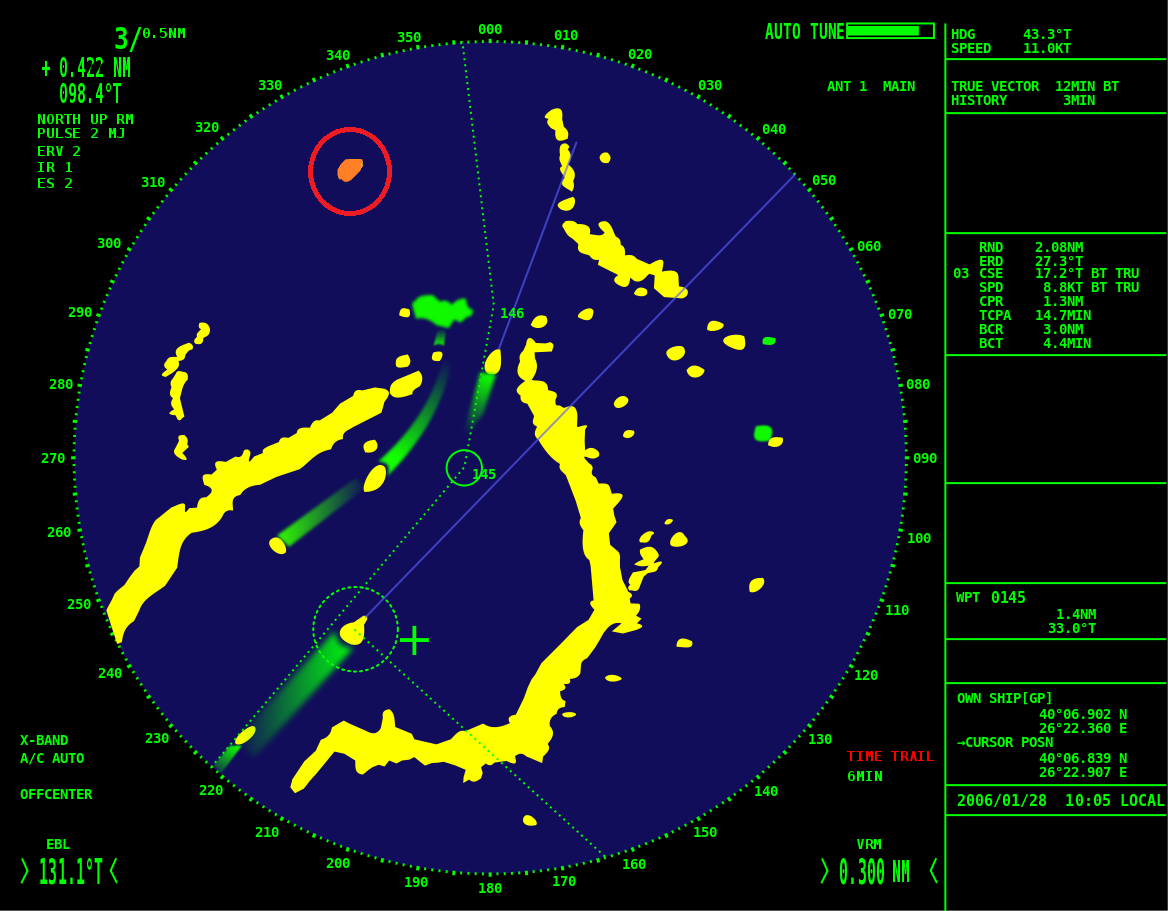
\includegraphics[width=\textwidth]{radarOrig2}
        \caption{Differentiated virtual object}
        \label{fig:five over x}
    \end{subfigure}
    \caption{Display of virtual objects on radar}
    \label{fig:three graphs}
\end{figure}

\section{Envisioned Technology}
\label{sec:envisionedtech}
An important choice in the design of a new human-computer interface is the technology used to build prototypes, and eventually the end product. For example, devices like keyboard, mouse and trackpad have acted as the standard input interface for personal computers for over 2 decades now, while computer monitors in the form of CRT, LCD and TFT displays have formed the output interface. Not unlike television monitors, computer monitors were initially used for purposes of data processing before being used for entertainment purposes such as gaming and media streaming. With the evolution of computing technology from large machines driven by punch cards and that filled up entire rooms to the personal computer form has coincided with their ubiquitous use in the modern world influencing the manner in which most office jobs are carried out today. 

Computers had a significant impact on the maritime industry. Where naval architecture was traditionally a craft with little scientific information to back designs, modern computers enabled computing power to be leveraged to predict performance. Modern ship designs make use of tools that have been developed to assess static and dynamic stability, water resistance, for hull development and structural analysis. Among other uses, maritime industry found use for computers as devices that could be used for the simulation of movements of vessels on sea. In a gaming-like use case, computers are used to run ship simulation software for educational purposes. These programs can be used to control virtual ships in virtual marine environments. Some setups involve actual bridge equipment to input commands to the program, making the experience more real-like. An array of monitors are used for display. Backed by computer graphics and models of sea, vessel and other objects, the simulation software is supposed to create the perception of being inside a real vessel. It is now standard practice to undergo training using simulators in the maritime industry. Figure \ref{fig:vstepdpsim} shows the setup of a typical dynamic positioning simulator. 


\begin{figure}
	\centering
	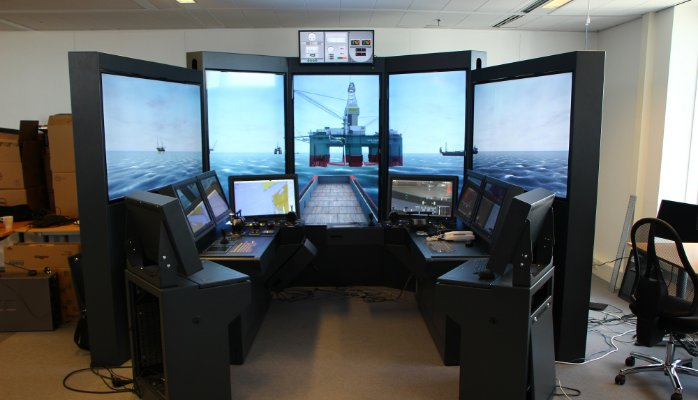
\includegraphics[width=\linewidth]{vstepdpsim}
	\caption{Setup of a dynamic positioning simulator by VSTEP}
	\label{fig:vstepdpsim}
\end{figure}


\subsection{Augmented Reality Display}
\todo{state conclusion here (going to use optical see through}
This section talks about display technology that is needed to create augmented reality applications.%creation of visual perception of mixed reality using digital display technology.
It briefly describes technological options available for augmented reality applications from the point-of-view of creating the visual perception that is part of augmented reality. Three ideas of mixed reality displays are considered, namely, optical see-through, video see-through head-mounted displays and, spatial augmented reality. Having been conceived in the 1980s, military and medical visualization contexts, these options for mixed reality displays were first catalogued in a landmark survey paper on augmented reality by Ronald Azuma \parencite{azuma1997survey}. 

The utility of different categories of augmented reality displays in the ship handling training context is considered in this research. Optical see-through displays theoretically allow an unhindered view of the outside world, whereas in video see-through display it is camera-mediated. Optical see-through HMDs appear to be the most logical choice for AR intuitively. It is ideologically consistent with AR in that most of the visual reality is left untouched, only to add bits of information (real/virtual) as necessary. Spatial augmented reality is another option for AR, but lack of mobility makes it infeasible in this scenario. It is nevertheless described in brief here for posterity. The following sections describe each of the display technologies in turn before comparing optical and video see-through HMDs. 

\subsubsection{Optical See-Through Head-Mounted Display}
Optical see-through head-mounted displays are one of the two basic choices available for mixed reality content display along with video see-though head-mounted displays. In general, see-through displays allow the user to see the real world through a display system while also being able to seamlessly display digital content on it. These were first developed for military aircraft for applications such as fixing the target of ammunition on locations that could be seen through the aircraft. The concept of see-through display is also making way into consumer markets, with head up displays used in cars being one of the more popular uses. Such display systems can also be mobile with users wearing them on the head so as to directly influence their view of the outside world. These are called as head-mounted displays. The following sections describe optical and video see-through displays in turn. A comparison of the two technologies on various parameters is presented thereafter.

Optical see-through head-mounted displays (OST) are display systems that exploit the transparency of glass material to provide unobstructed views of the outside world. By definition, they can also digital content on the same surface simultaneously. As figure \ref{fig:opticalseethrough} shows, OST displays use optical combiners to combine light from the real world with that of the digital content. Optical combiners usually reduce the amount of light from real world. Combiners act like half-silvered mirrors to be able to reflect light from monitors into user's eyes. Theoretically, this display system can provide undistorted view of the real world (apart from slight obstructions caused by the frame itself). As a downside, it also affects the display of digital content adversely, making virtual objects appear semi-transparent and 'ghostlike'.

\begin{figure}
	\centering
	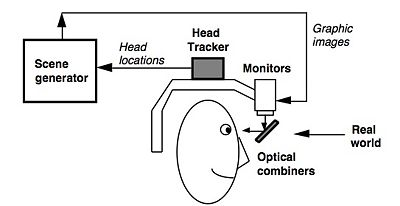
\includegraphics[width=\linewidth]{opticalseethrough}
	\caption{Schematic diagram of optical see through display (Source: \cite{azuma1997survey})}
	\label{fig:opticalseethrough}
\end{figure}

\subsubsection{Video See-Through Head-Mounted Display}
Video see-through HMDs are similar to optical see-through HMDs in that they allow the combination of real world views with digital content. Differences between them stem from their source of real world view. As opposed to OST which provides a direct view of the environment, VST uses video feed from a camera in the HMD system to provide real world views. So, in addition to the head trackers and viewing monitors as in OST HMDs, VST HMDs require a camera appendage in the setup (see figure \ref{fig:videoseethrough}). This type of HMDs block the wearer's external view in favor of better immersion into the stereoscopic view provided by the system. A video camera can be mounted on the exterior of such an HMD to incorporate external view back into the content.
%\todo[inline]{consider revision}

Driven by interest from the gaming community, and virtual reality applications in general, closed-view HMDs have seen more development as of this writing. Low cost HMDs are available in the consumer market, and can be used for 3D games and entertainment applications. With the addition of one or two cameras, these can be leveraged for mixed reality applications. Consequently, calibration of the camera's view to that of the user's eye position will have to be made.

\begin{figure}
	\centering
	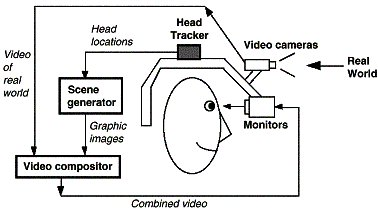
\includegraphics[width=\linewidth]{videoseethrough}
	\caption{Schematic diagram of video see through display (Source: \cite{azuma1997survey})}
	\label{fig:videoseethrough}
\end{figure}



\subsubsection{Spatial Augmented Reality}

Spatial augmented reality (SAR) refers to the concept of augmenting real-world spaces (with digital media) without the use of special devices such head-mounted display. As an AR technology, implementations of SAR must adhere to the basic requirements of augmented reality listed in section \ref{sec:augreal}. Along with HMDs, it forms another paradigm for the creation of mixed reality content. SAR offers unique benefits over HMDs such as obviating the need to wear special devices and possibly high resolution, wide field of view displays integrated into natural environments. Large field of view and higher resolution provides a stronger feeling of presence \parencite{lantz1996future}, allowing for better immersion and easier eye accommodation\footnote{refer to section \ref{sec:photorealism} for a discussion on photorealism}. On the downside, it suffers from setbacks such as having to set up expensive custom-made display configurations that require more space and hardware than standardized HMDS. 

The lack of standardized solutions and the need to setup special hardware tailored to individual ships makes SAR an impractical solution for creation of AR onboard ships for maneuvering training purposes. A portable technological solution that enables mobility between vessels is desired. This allows for trainings to be conducted on various different vessels with minimal time and effort involved in setting up the augmented environment. Instead, the use of mobile AR devices such as HMDs means that trainees can carry individual AR devices onboard and vessels do not need to be docked for purposes of setting up the AR environment. Nevertheless, the concept is described in brief here for completeness. A detailed treatment of the topic of spatial augmented reality can be found in \cite{bimber2005spatial}.

Figure \ref{fig:monitorseethrough} shows a concept of monitor-based spatial augmented reality. In this setup, the user views the mixed reality on one or more monitors in front of the user which display a combination of virtual and real world images captured by video camera. This is similar to the CAVE \parencite{cruz1993surround} concept for virtual reality. CAVE (CAVE automatic virtual environment) seeks to immerse the user in a 3D virtual environment created using rear/front facing projectors lighting up projection screens in 3 dimensions. Although originally designed for virtual reality experience, the concept can be adapted for augmented reality. Advances in projection technology make it possible to have projections on transparent screens \parencite{peterson2006human}. 

\begin{figure}
	\centering
	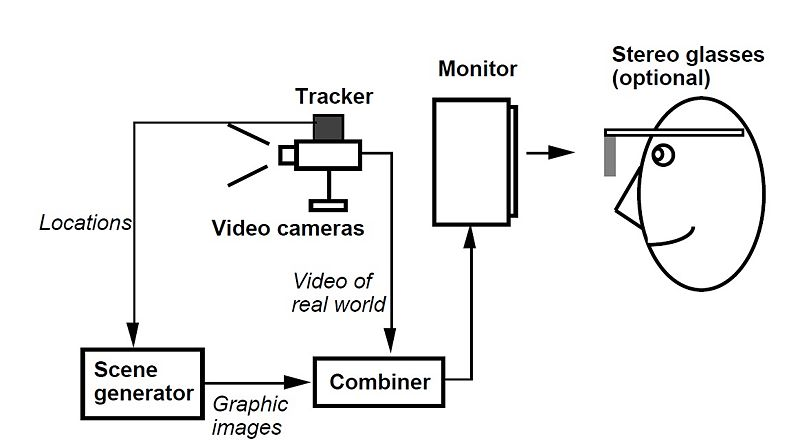
\includegraphics[width=\linewidth]{monitorseethrough}
	\caption{Schematic diagram of monitor see through display (Source: \cite{azuma1997survey})}
	\label{fig:monitorseethrough}
\end{figure}

A discussion of display options for AR would be incomplete without spatial augmented reality. As opposed to head-mounted displays, SAR relies on projectors to create the views necessary for the perception of mixed reality. SAR may be just as effective as head-mounted displays in being able to create immersive mixed environments. A study on the use of large projection screen as an alternative to HMDs for virtual environment found no significant difference between the two for spatial cognition tasks \parencite{patrick2000using}. But projector-based display systems are custom solutions that need to be designed for the specific environment in consideration. Ships come in a variety of shapes and sizes, so do their bridge rooms. Setting up MR environments onboard different supply vessels would then involve considerable effort to tailor the display system for individual ships. Besides, some modification of the ship bridge room is involved such as placing projectors at the appropriate locations and turning bridge windows in to projection screens onto which virtual objects can be projected.

\subsection{Comparison of Head-Mounted Displays}
This section provides a comparison of optical and video see-through HMDs based on parameters thought to be relevant to this study. For an in-depth review and comparison between these two display types, readers can refer to \cite{rolland1995comparison}.

\begin{enumerate}
\item \textit{Simplicity}: In mixed reality applications, there is a need to see the external world besides virtual images being displayed in the HMDs. Optical see-through systems meet this requirement naturally from employing transparent displays which do not interfere with the external view. Video see-through systems on the other hand, use a camera to capture the external view. The camera then seeks to perform the role of human vision, one of the most complicated sensory systems in the universe, the various functions of which are either not built into or not yet achievable using consumer grade cameras. For example, the resolution of the entire view (real + virtual) is limited to that of the display device in case of VST. This constraint is also present in optical see-through devices, with a crucial difference that it is only applicable to virtual parts of the scene. 

\item \textit{Lag}: A persistent problem with interactive computer graphics is that of time delay (lag) between expectation of the appearance of a scene and it's actual appearance. For example, in an OST system, there will be near zero lag in viewing real scene as it is viewed directly by the user. Whereas, the display of any virtual objects can be a source of lag. The system first needs to decide whether to display virtual objects based on viewing direction and orientation and, also calculate appropriate projection of the virtual object if it needs to be displayed indeed. Finally, there will be a small delay in rendering the images itself. 

In case of video see-through systems, additional lag is present from having to digitize video stream of the real world. In a display that refreshes at 60Hz, the time that elapses between display of one frame and another is 16.67ms. Hence there will be a minimum of 16.67ms delay in displaying the external view recorded by a camera, discounting the time taken to digitize the camera view. According to \parencite{ellis1997factors}, for close range tasks, one millisecond of delay causes one millimeter of error

An advantage of VST over OST is that the higher degree of control over display streams (real and virtual) in video see-through makes it possible to avoid the problem of temporal mismatch due to delay in virtual images by delaying real view as well. 
 
\end{enumerate}

\begin{table}[]
\centering
\caption{Comparison of see-through head-mounted displays}
\label{tab:comparehmds}
\begin{tabular}{@{}p{3.5cm}|P{4.5cm}|P{4.5cm}@{}}
\toprule
                                           & \multicolumn{1}{P{4cm}|}{\textbf{Optical see-through}}                          & \multicolumn{1}{P{4cm}|}{\textbf{Video see-through}} \\ \midrule
Simplicity                                 & Only one stream to process (virtual images)                            & Two streams to process (camera feed + virtual images)                                                         \\
\hline
%\todo{add comparison of calibration and registration}
%Calibration                                & Need to calibrate for user's unique facial geometry and facial acuity. & Availability of single digital composite of real and virtual images allows use of computer vision techniques. \\
Quality of real world view                 & Largely undistorted                                                    & Camera and display dependent                                                                                   \\
\hline
Time lag of real world view                & 0ms                                                                    & \textgreater 16ms                                                                                              \\ 
\hline
Resolution                                 & Partially display dependent                                            & Fully Camera and display dependent                                                                             \\
\hline
Peripheral field of view (horizontal)      & 180 degrees                                                            & 110 degrees                                                                                                   \\
\hline
Digital display field of view (horizontal) & 20-40 degrees                                                          & \textgreater 90 degrees                                                                                        \\
\hline
Focus and contrast                         & Hard to blend virtual object into real scene                           & Less severe contrast issues due to limited dynamic response of cameras                                        \\
\hline
Occlusion                                  & Challenging to achieve full occlusion									& Occlusion is possible due to full control over displayed content \\ \bottomrule 
\end{tabular}
\end{table}

The display technologies considered so far have been applicable for creation of mixed reality for individual users. These systems do not scale easily to groups of users needing to experience the same mixed reality. For example, in the mixed reality ship handling training method that is being conceived in this project, it is required that at least two people experience the same scenario, i.e. the trainee and a trainer (experience ship handler). Apart from the trainee who needs to view the virtual object/s for training purposes, the trainer also needs to see the same in order to evaluate trainee performance. Collaborative design such as for architecture and modeling is another use case multiple users needing to experience the same mixed reality. 

\subsubsection{Photorealism}
\label{sec:photorealism}

\begin{table}[h]
\centering
\caption{Levels of photorealism}
\label{tab:trainingoptions}
\begin{tabular}{@{}P{2.5cm}p{10cm}@{}}
\toprule
\multicolumn{1}{P{2.5cm}}{\textbf{Classification}} & \multicolumn{1}{p{10cm}}{\textbf{Reasoning}} \\ 
\hline
High & \vspace{-2mm} \begin{enumerate}[leftmargin=*,topsep=0pt,partopsep=0pt,align=left,itemsep=0.05cm]
\item Presentation of occlusion, a basic depth cue, is necessary to induce sense of depth in the augmented scene
\item Wide field of view is required to create illusion of large object being nearby.	
\item  Virtual object is the main focus in the scene and, inconsistency in 3D view of augmented reality can hamper task performance from visual fatigue due to accomodation-vergence conflict.
\end{enumerate}
\vspace{-\baselineskip}\\
\hline
Medium & \vspace{-2mm} \begin{enumerate}[leftmargin=*,topsep=0pt,partopsep=0pt,align=left,itemsep=0.05cm]
\item Occlusion is useful to induce depth in the scene, but some amount transparency can be tolerated.
\item  Lack of wide field of view does not affect task performance. 
\item  Inconsistency in 3D view does not easily amount to visual fatigue as virtual object is not the user's main object of focus in the augmented scene.
\end{enumerate}
\vspace{-\baselineskip}\\
\hline
Low & \vspace{-2mm} \begin{enumerate}[leftmargin=*,topsep=0pt,partopsep=0pt,align=left,itemsep=0.05cm]
\item Depth cues in the scene are not necessary for purposes of the training.
\item Wide field of view is not required for effective task performance.
\item Inconsistency in 3D view does not easily amount to visual fatigue as virtual object is not the user's main object of focus in the augmented scene
\end{enumerate}
\vspace{-\baselineskip}\\
\bottomrule
\end{tabular}
\end{table}

\subsection{Ship Instrument Augmentation}

Mixed reality displays described in the previous section form a part of enabling technologies for the mixed reality ship maneuvering training conceptualized in this research. HMDs for instance can help create visual perception of an offshore oil platform standing on the open sea. In other training scenarios they may be used to display tracks/lanes for navigational tracking or virtual ships on collision course/sailing side-by-side etc. Different artifacts may be displayed depending on training objectives and the perceptions that need to be created. Ships over the years though have evolved to be technically complex machines. The bridge room of a modern age vessel houses multiple instruments tracking different aspects of its reality. Therefore, the design of a mixed reality environment on-board a modern seafaring vessel should consider how virtual objects interact with various instruments in the bridge room to accurately correspond with the reality that is being visually perceived.  

\subsubsection{Bridge Instrumentation}



\subsubsection{Tracking Requirements}

\paragraph{In-out vs out-in tracking}

\paragraph{Fiducial Markers}
